\documentclass[border=2pt]{standalone}
\usepackage{pgfplots}
\pgfplotsset{compat=1.18}
\begin{document}
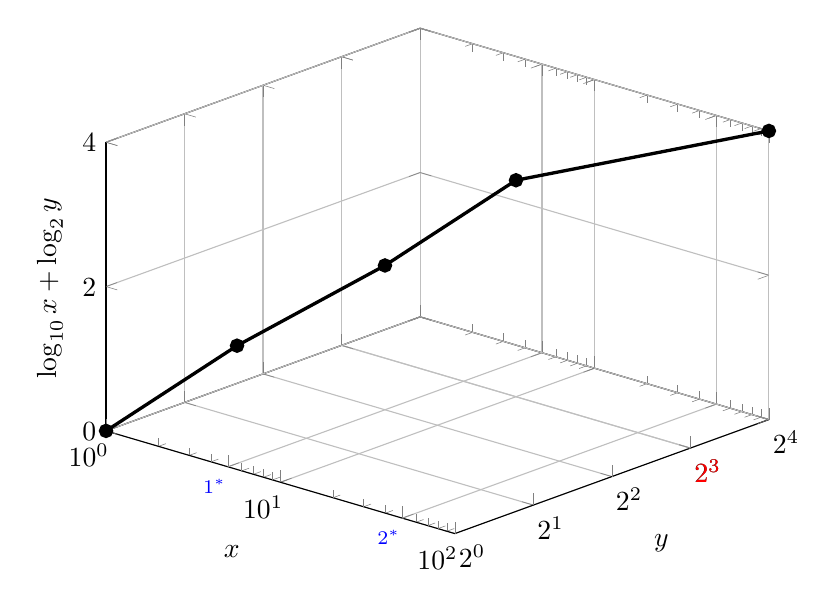
\begin{tikzpicture}
  \begin{axis}[
    width=10cm,
    height=8cm,
    view={42}{28},
    xmode=log,
    ymode=log,
    log basis x=10,
    log basis y=2,
    xmin=1,xmax=100,
    ymin=1,ymax=16,
    zmin=0,zmax=4,
    grid=major,
    xlabel={$x$},
    ylabel={$y$},
    zlabel={$\log_{10}x+\log_2y$},
    extra x ticks={5,50},
    extra x tick label={${\pgfmathprintnumber[fixed,precision=0]{\tick}}^*$},
    extra x tick style={tick label style={text=blue,font=\scriptsize}},
    extra y ticks={8},
    extra y tick labels={$2^3$},
    extra y tick style={tick label style={text=red}}
  ]
    \addplot3[very thick,mark=*] coordinates {
      (1,1,0) (2,2,1) (5,4,2) (10,8,3) (100,16,4)
    };
  \end{axis}
\end{tikzpicture}
\end{document}
